\chapter{Resonance Compensation Studies at the CERN Proton Synchrotron Booster}
\label{sec:ch5}

\section{General Description}
The Proton Synchrotron Booster (PSB) is the first circular accelerator in the CERN accelerator complex that ultimately leads to the LHC. Figure \ref{fig:cernac} shows the entire chain of accelerators at CERN, feeding a variety of physics experiments \cite{cernplot}. Following the successful implementation of the LHC Injectors Upgrade (LIU) \cite{liu}, the PSB receives $H^-$ ion beam coming from the Linac4 at an energy of 160 MeV. Interestingly enough, the PSB is not just one ring, but rather four identical synchrotron rings stacked on top of each other. This is to counteract space charge effects which are largest at low energy machines. Once the ion beam enters the PSB rings, the electrons are stripped off through a charge-exchange process with a carbon foil and proton beam is achieved \cite{psbstrip}. The proton beam is then accelerated from an energy of 160 MeV to 2 GeV. The beam from the four rings gets merged together and then gets injected to the Proton Synchrotron (PS). This is true for LHC-type beams, nevertheless, the PSB can also accelerate lead ions and deliver to other customers such as the heavy ion experiments, e.g., ISOLDE \cite{foteini1}.   

One ring of the PS Booster has a total circumference of 157.08 meters. Multiplying this quantity by the four rings you get a length of 628.32 meters, which is the exact circumference of the next accelerator, the Proton Synchrotron (PS). The PSB has a superperiodicity of 16, meaning it has 16 identical fundamental cells. Each cell has a length of 9.82 meters housing a sequence of bending magnet, focusing quadrupole, defocusing quadrupole, focusing quadrupole and bending magnet \cite{tirsithesis}. In between these main components there are drift spaces used for RF insertions, diagnostic devices, injection and extraction devices and additional multipole corrector magnets. At injection energy, 160 MeV, protons have a revolution period of 1.01 $\mu s$, while at the extraction energy of 2.0 GeV they have a revolution period of 0.553 $\mu s$. The overall cycle in the PS Booster takes around 1.2 seconds. 

\begin{figure}[H]
    \centering
    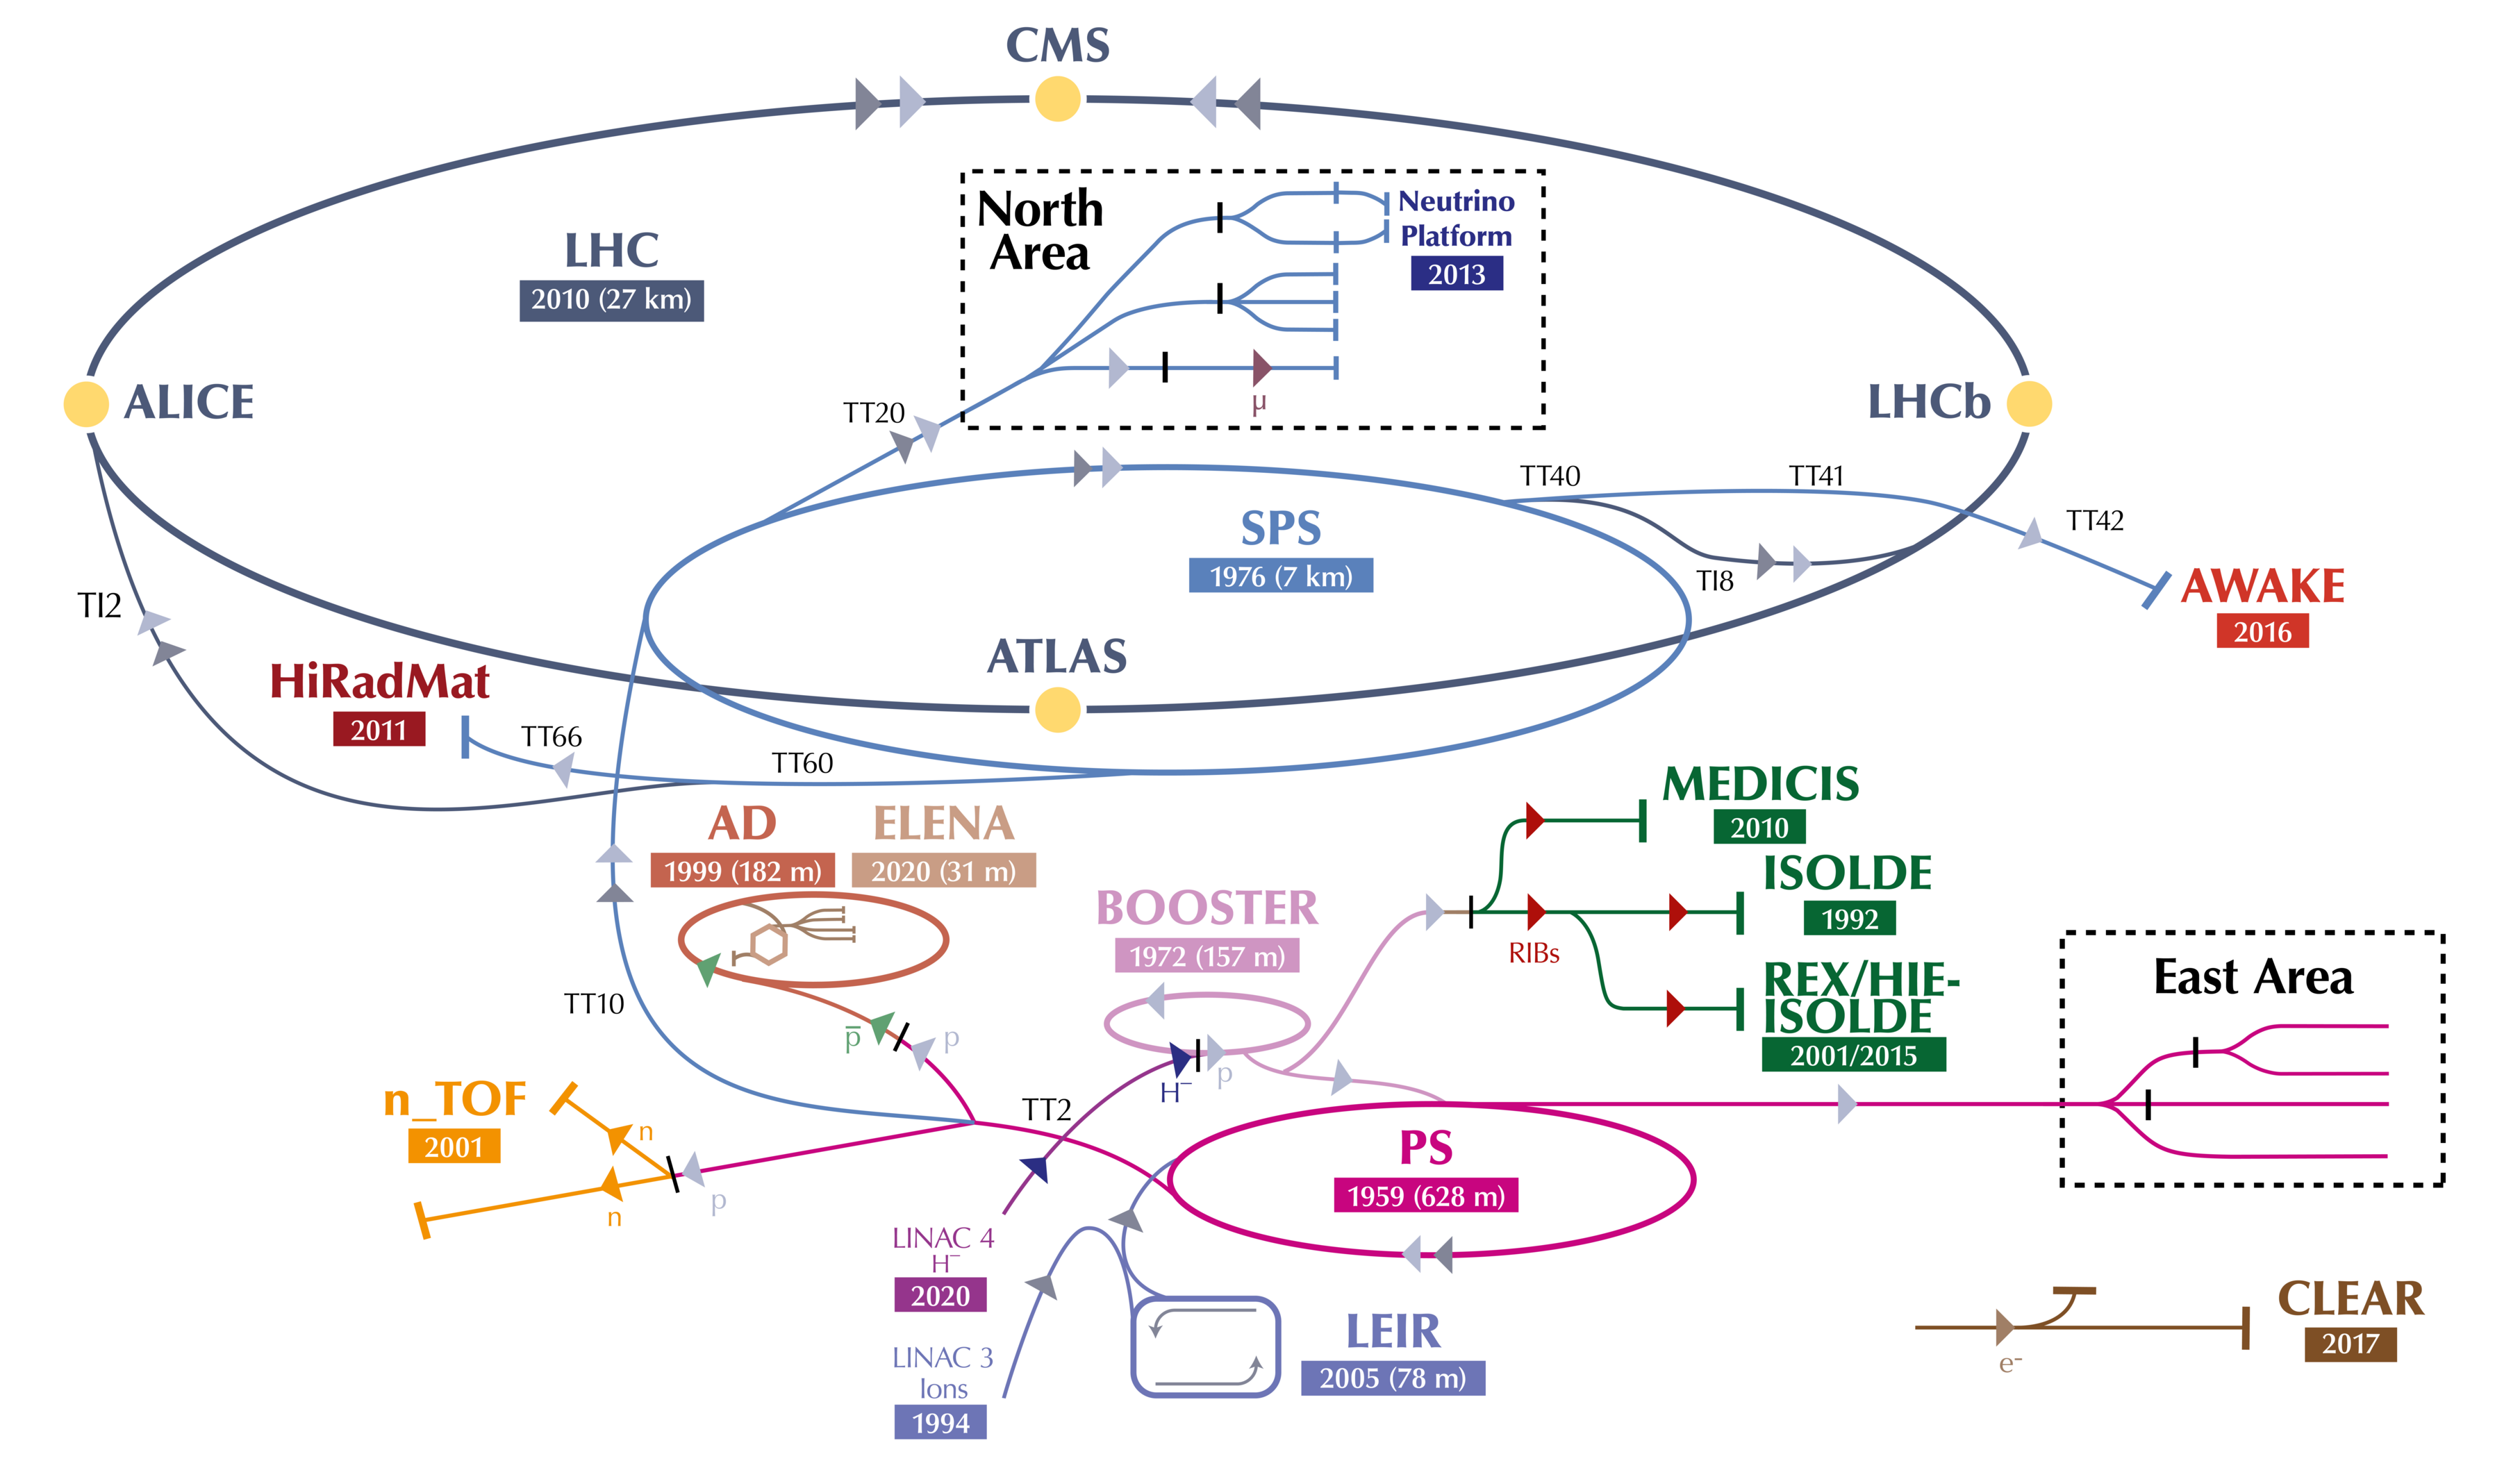
\includegraphics[width=\linewidth]{chapter5/CERN_AC.png}
    \caption{A graphic overview of all accelerators in operation at CERN as of 2022. Original image taken from Ref. \cite{cernplot}. This file is licensed under the Creative Commons Attribution 4.0 International license.}
    \label{fig:cernac}
\end{figure}

\section{Tune Diagram and Operation}

Figure \ref{fig:operational_psb} illustrates the tune diagram dynamics that LHC-type beam undergoes at the PS Booster \cite{foteini1,foteini2,albright}. As mentioned before, beam gets injected at an energy of 160 MeV. At this low energy, the tune footprint is large enough that the spread can reach values of up to 0.5, i.e., $\Delta Q_u \approx -0.5$. The nominal injection tunes are around $Q_x = 4.40$ and $Q_y = 4.45$, in order to accommodate the footprint between the integer resonance lines $Q_u= 4.0$ and the half-integer line $2Q_y=9$. As the beam is accelerated, the quadrupoles are ramped up to match the increasing beam rigidity, but, additionally, a tune ramp is introduced in order to move the shrinking footprint to a less resonance-populated area in the tune diagram. The nominal extraction tunes are around $Q_x = 4.17$ and $Q_y = 4.23$. At extraction, the beam tune footprint has shrunk by a factor of $(\gamma_L ^3 \beta_L ^2)$, as explained by the beam perveance definition in Eq. \ref{eq:perv}. At extraction, the footprint is smaller than 0.05, i.e., $| \Delta Q_u | \lesssim 0.05$.      

\begin{figure}[H]
    \centering
    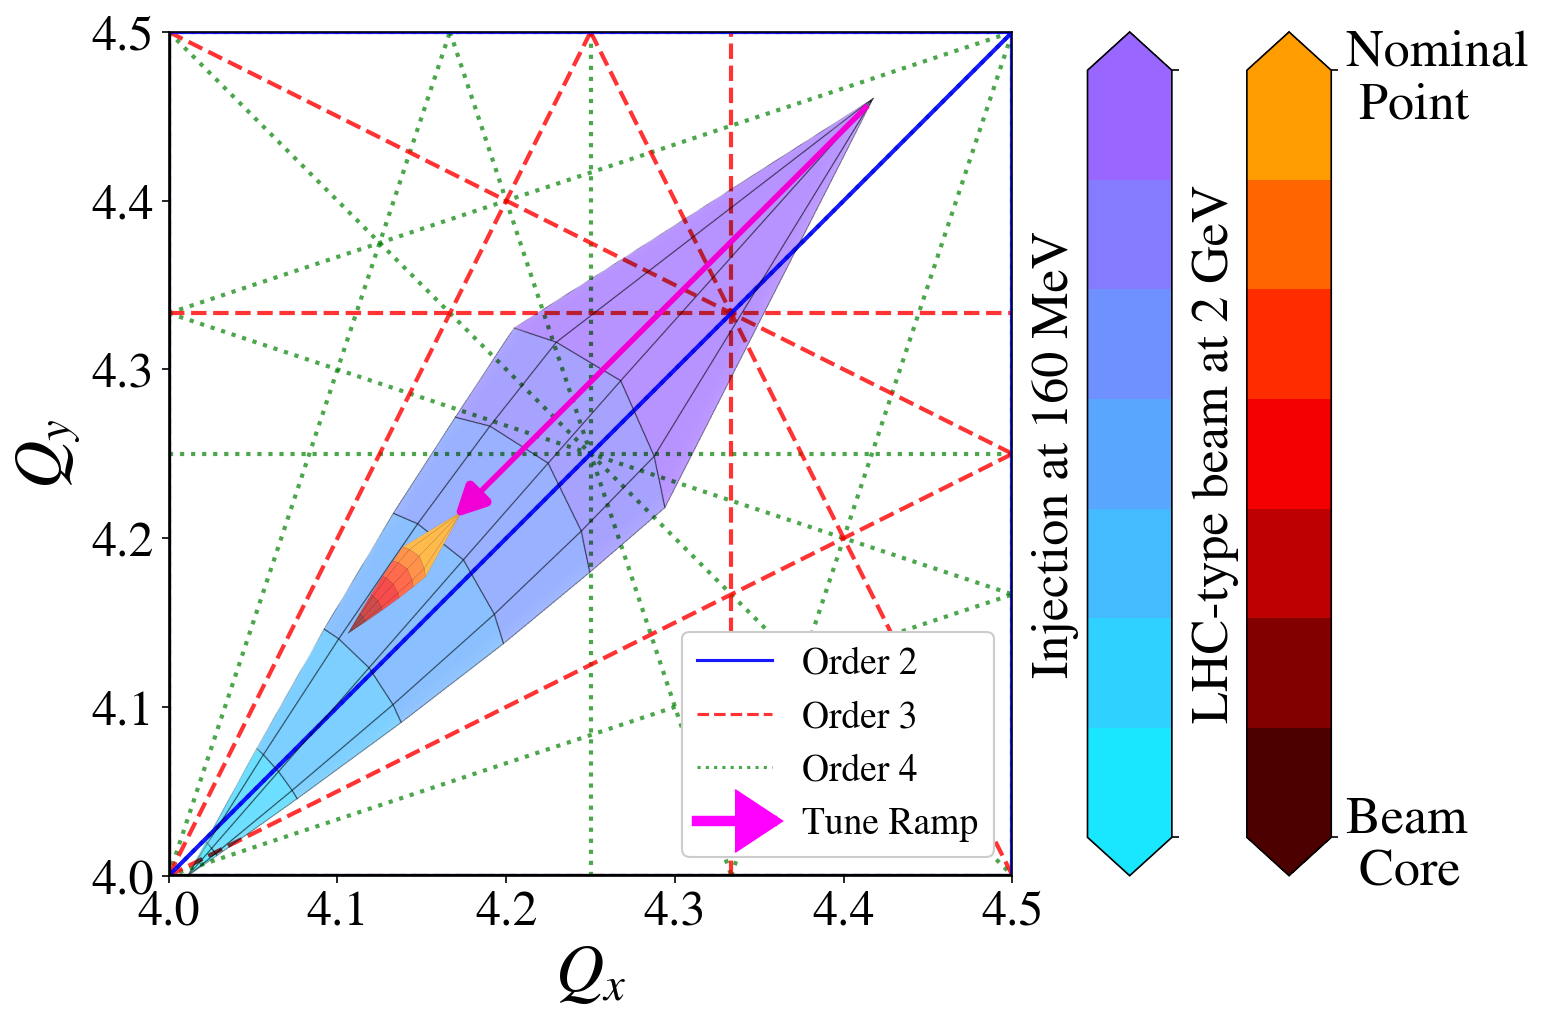
\includegraphics[width=\linewidth,keepaspectratio]{chapter5/operational.png}
    \caption{Operational tune footprint for PSB beam at injection (cool color map) and footprint after beam has been accelerated to 2 GeV (warm color map). During acceleration, there is a tune ramp illustrated with the fuchsia arrow.}
    \label{fig:operational_psb}
\end{figure}

The nominal tune ramp, as illustrated in Fig. \ref{fig:operational_psb} with the fuchsia arrow, crosses several resonance lines. These include 4 third-order resonance lines and 4 fourth-order lines. It is worth reminding the reader that the third order lines are excited by sextupole component in the ring, while fourth-order lines are excited by octupole fields in the ring. The third order resonances include two normal sextupole lines, $3Q_x = 13$ and $Q_x+2Q_y = 13$, and two skew sextupole lines, $3Q_y = 13$ and $2Q_x+Q_y = 13$. For the octupole case, these include two normal octupole lines, $4Q_x = 17$ and $Q_x+3Q_y = 17$, two skew octupole lines, $4Q_y = 17$ and $3Q_x+Q_y = 17$, and the octupole coupling sum resonance, $2Q_x +2Q_y =17$. Figure \ref{fig:psbtd} shows all of these resonance lines summarized in one tune diagram. All of these resonance lines have different strengths in each Booster ring. It is worth pointing out that the coupling resonance $Q_x - Q_y = 0$ is already being corrected for with skew quadrupoles, similar to the Recycler Ring case.   

\begin{figure}[H]
    \centering
    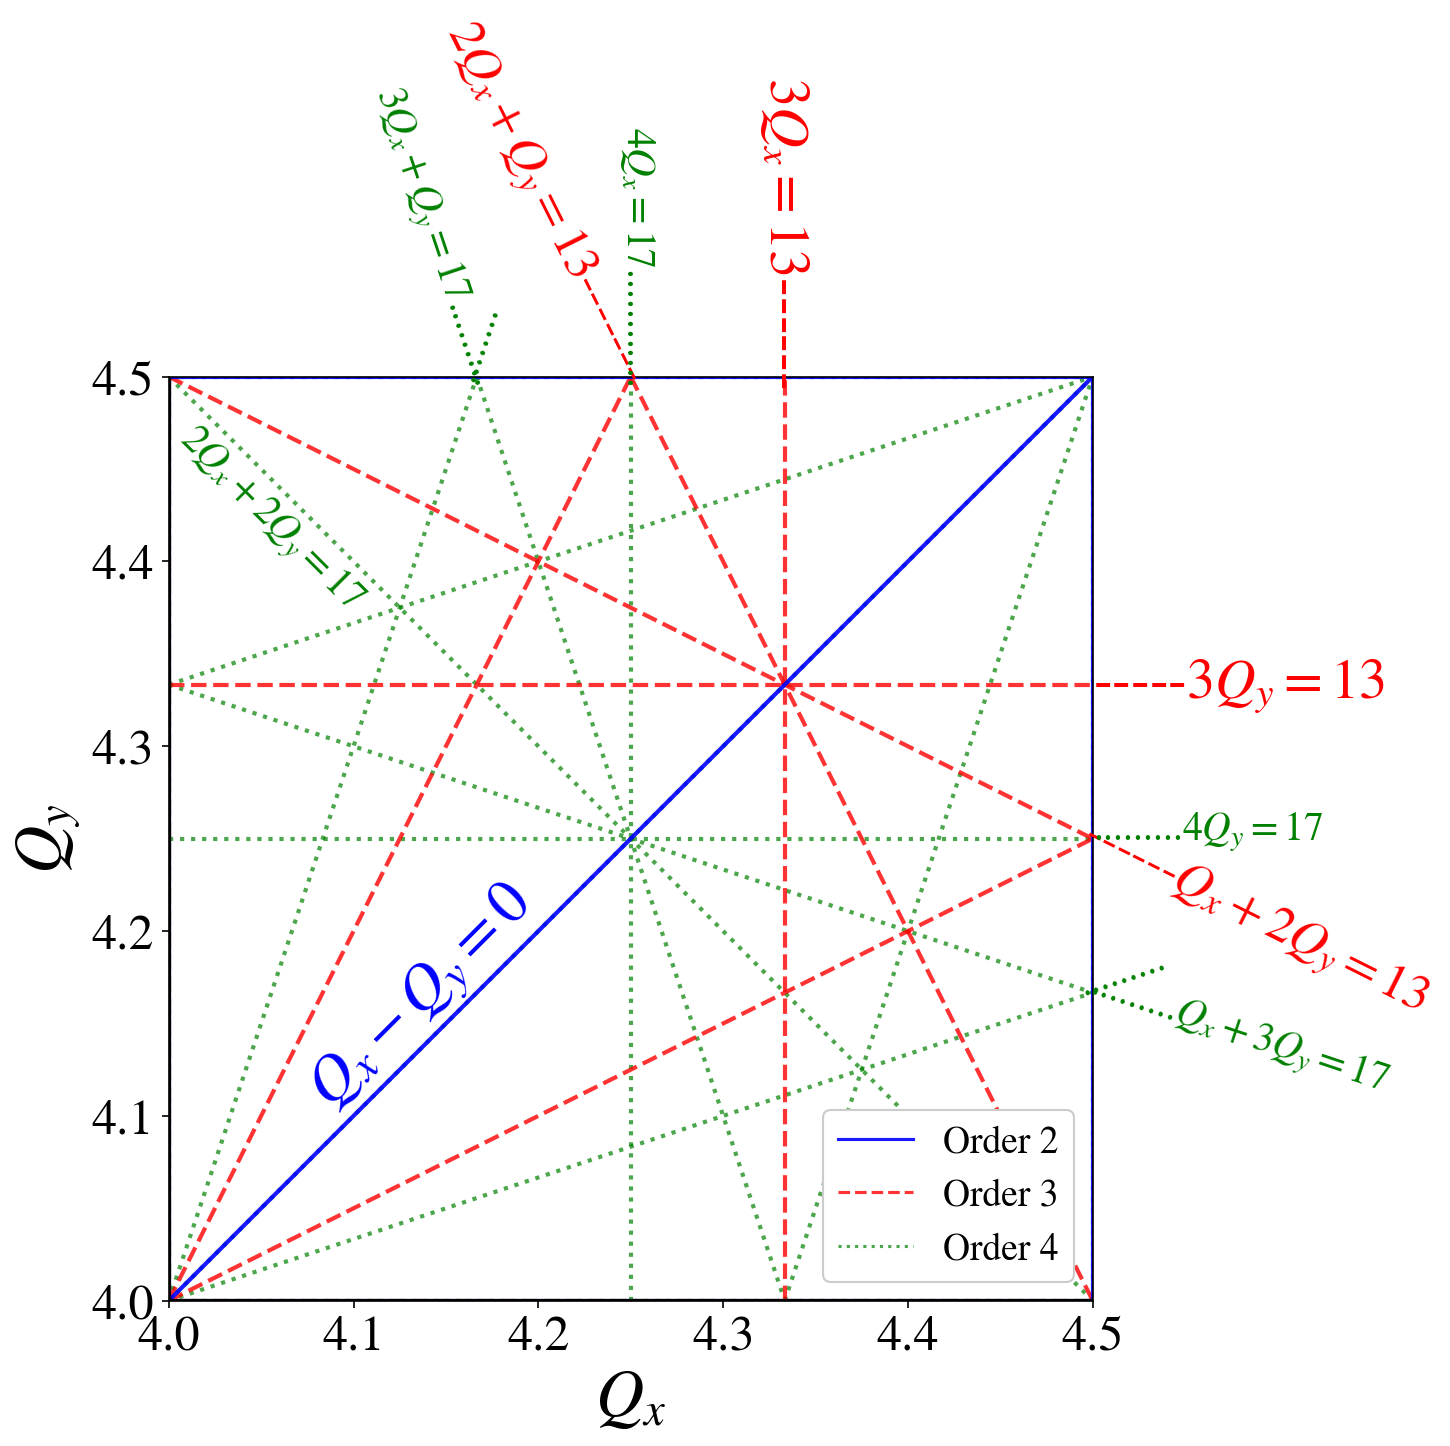
\includegraphics[width=\linewidth]{chapter5/psb_td.png}
    \caption{Portion of the tune diagram enclosing the operational tunes of the PS Booster with relevant resonance lines labelled.}
    \label{fig:psbtd}
\end{figure}

Similar to the plots shown in Fig. \ref{fig:bare_nocomments} and Fig. \ref{fig:bare_comments}, loss maps can be used to visualize the strength 

\begin{figure}[H]
    \centering
    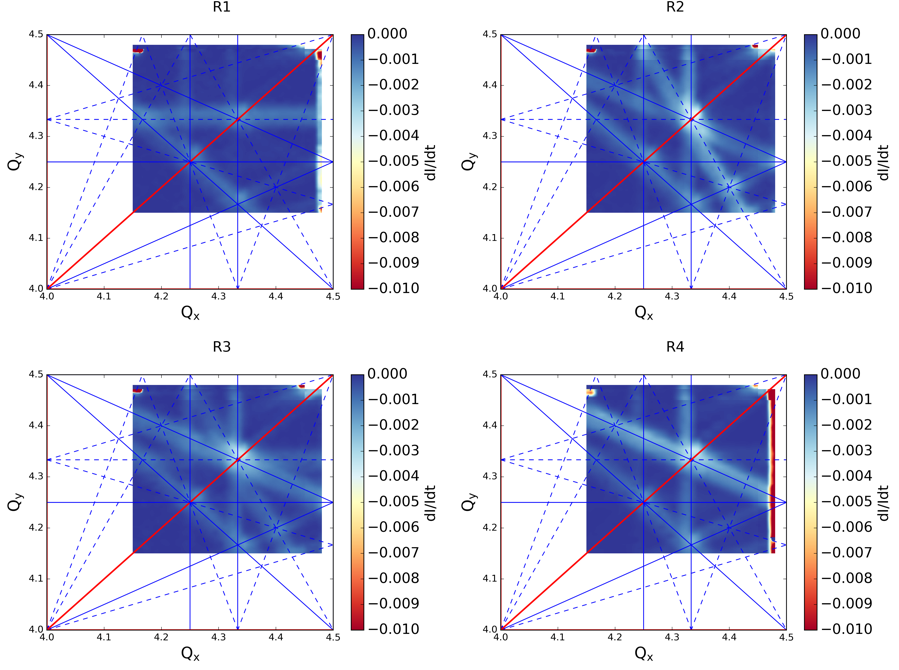
\includegraphics[width=\columnwidth]{chapter5/bare.png}
    \caption{Dynamic loss maps for the bare machine of the 4 rings in the PS Booster. The plots are an average of scanning in 4 directions.}
    \label{fig:bare_psb}
\end{figure}

\section{Optimization Algorithms for Resonance Compensation}

\cite{geoff} 


\begin{figure}[H]
    \centering
    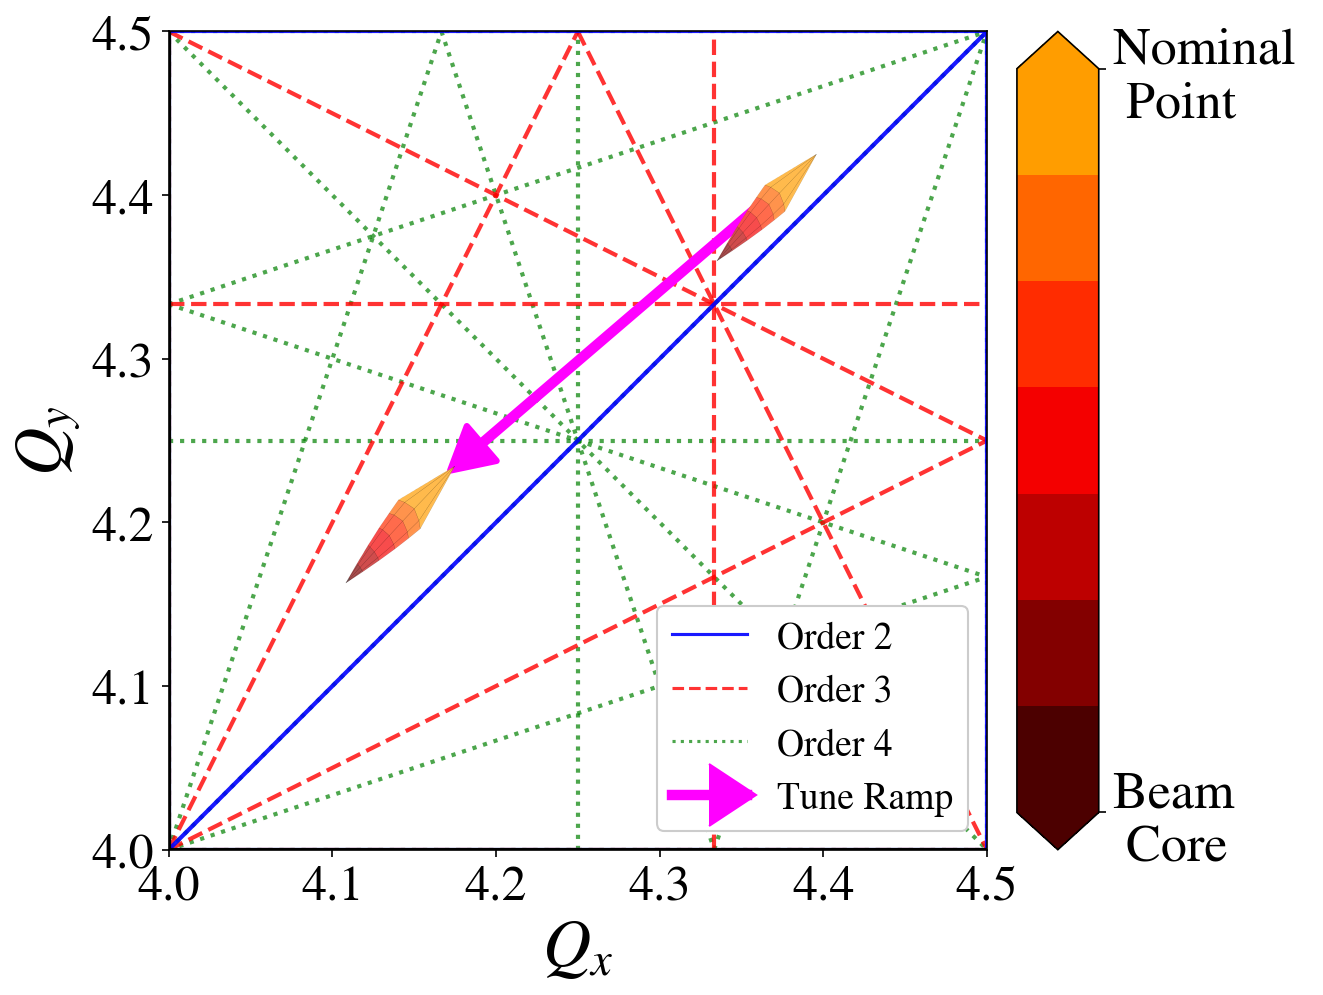
\includegraphics[width=\linewidth]{chapter5/experiment.png}
    \caption{Experimental setup of the tune diagram dynamics for the optimization of resonance compensation used in the PS Booster.}
    \label{fig:experimentPSB}
\end{figure}

\begin{table}[H]
    \centering
    \caption{List of elements (optimization actors) in the PS Booster at CERN used for resonance compensation optimization as present in all four PS Booster rings.}
    \label{tab:psbcomp}
    \begin{tabular}{|c|c|c|}
    \hline
    \textbf{Actor} & \textbf{Name} & \textbf{Type}    \\ \hline
    1 & XN04L1    & Normal Sextupole \\ \hline
    2 & XN06L1    & Normal Sextupole \\ \hline
    3 & XN09L1    & Normal Sextupole \\ \hline
    4 & XN012L1    & Normal Sextupole \\ \hline
    5 & XN0311L1    & Normal Sextupole   \\ \hline
    6 & XN0816L1    & Normal Sextupole   \\ \hline
    7 & ON0311L1    & Normal Octupole  \\ \hline
    8 & ON0816L1    & Normal Octupole   \\ \hline
    9 & XSK2L4    & Skew Sextupole  \\ \hline
    10 & XSK4L1    & Skew Sextupole   \\ \hline
    11 & XSK6L4    & Skew Sextupole   \\ \hline
    \end{tabular}
\end{table}

\begin{figure}[H]
    \centering
    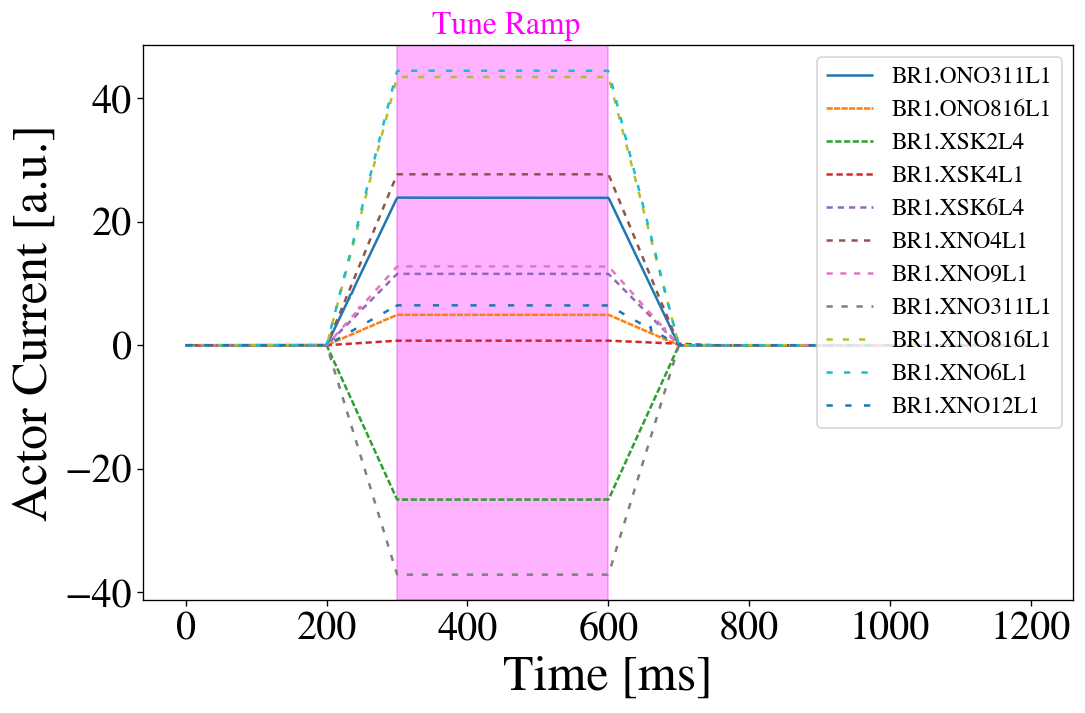
\includegraphics[width=\linewidth]{chapter5/actor_currents.png}
    \caption{Waveform for the currents fed to the correctors (actors) as a function of time in the study cycle}
    \label{fig:actorcurrents}
\end{figure}

\subsection{Bayesian Optimization}

\begin{figure}[H]
    \centering
    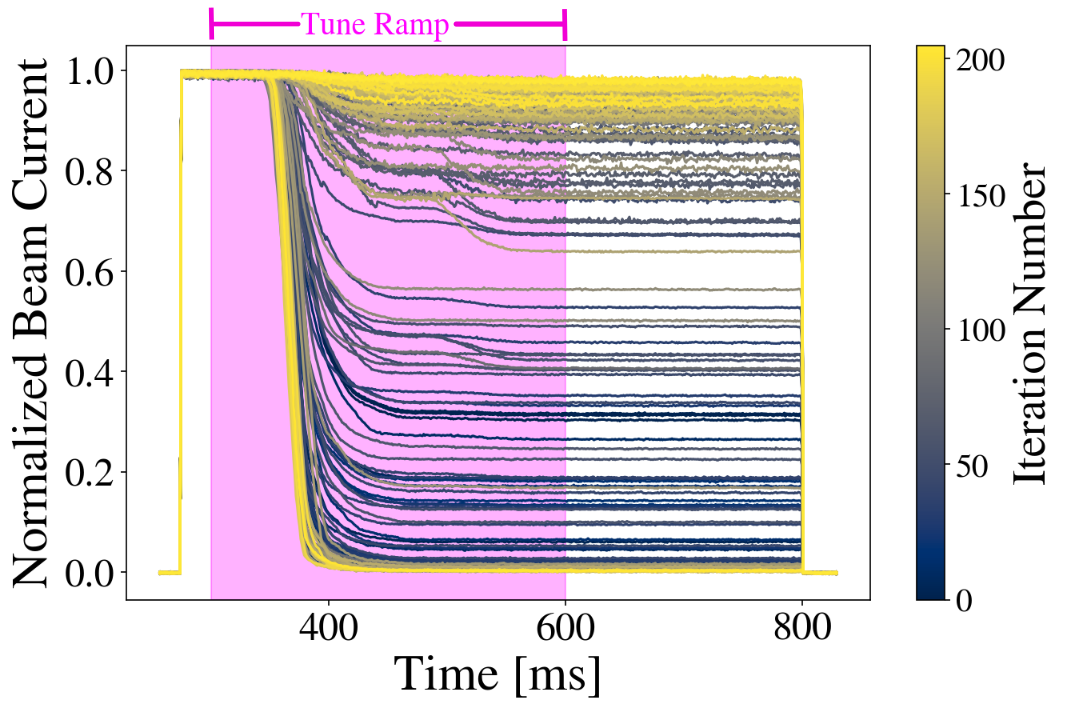
\includegraphics[width=\linewidth]{chapter5/i1_bo_commented.png}
    \caption{Normalized beam current plots for the Bayesian Optimization method done at Ring 1.}
    \label{fig:ibo}
\end{figure}

\begin{figure}[H]
    \centering
    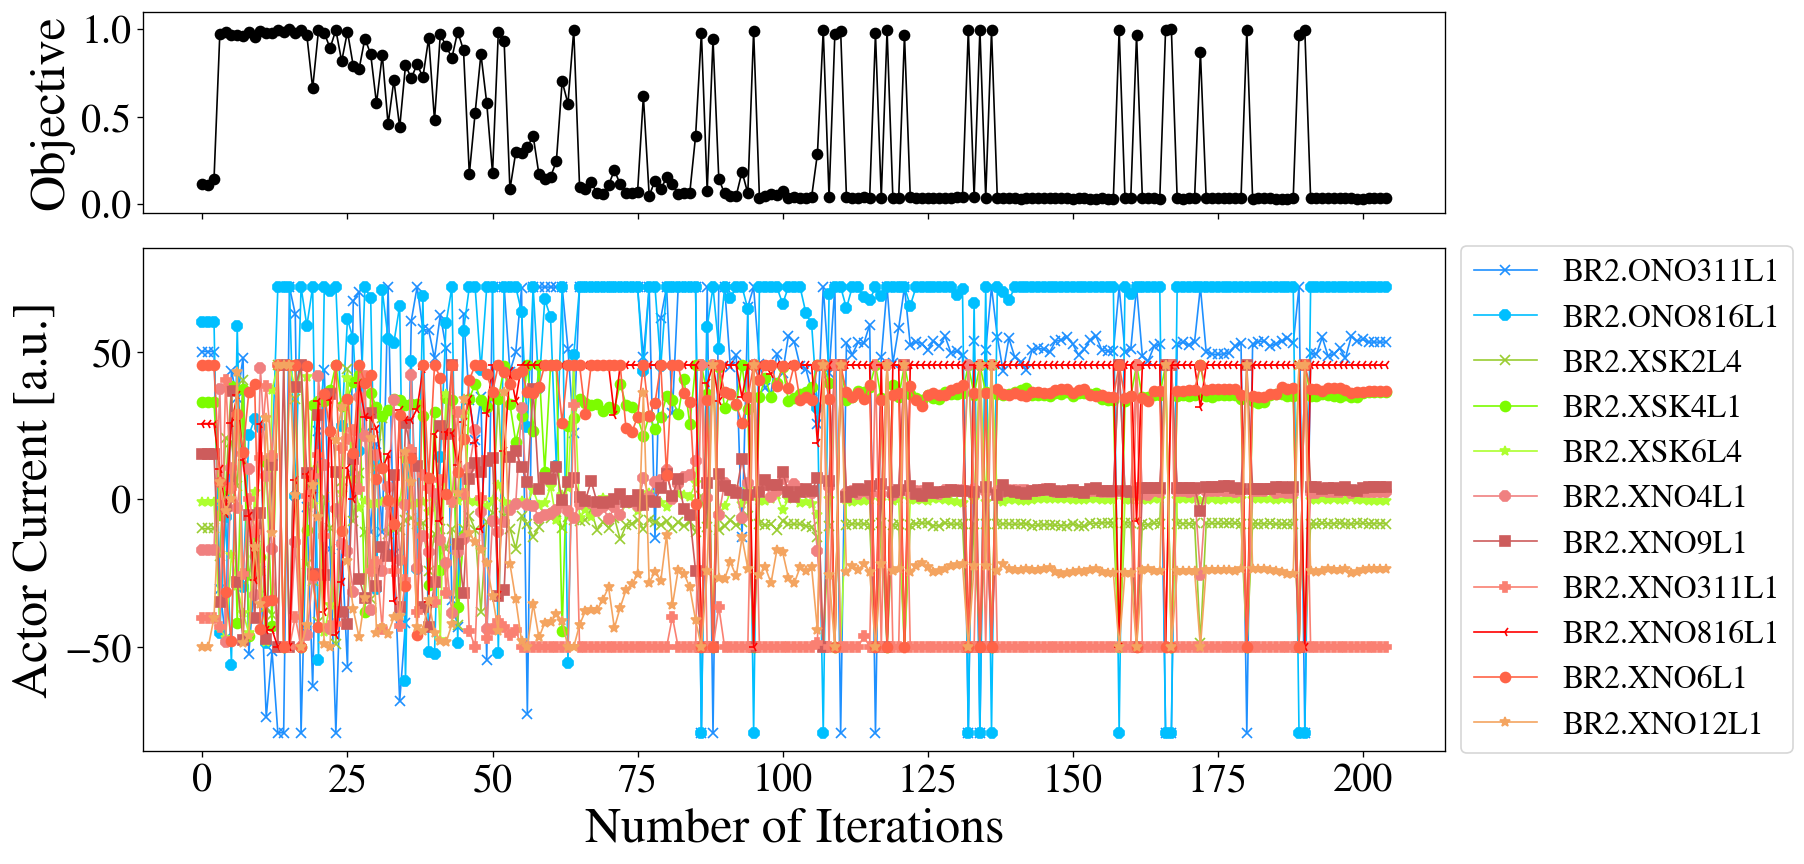
\includegraphics[width=\linewidth]{chapter5/2023_05_02_R2_LHCramp_BayesOpt.png}
    \caption{Summary for Bayesian optimization of resonance compensation applied to Ring 2 in the CERN PSB.}
    \label{fig:bo1}
\end{figure}

\begin{figure}[H]
    \centering
    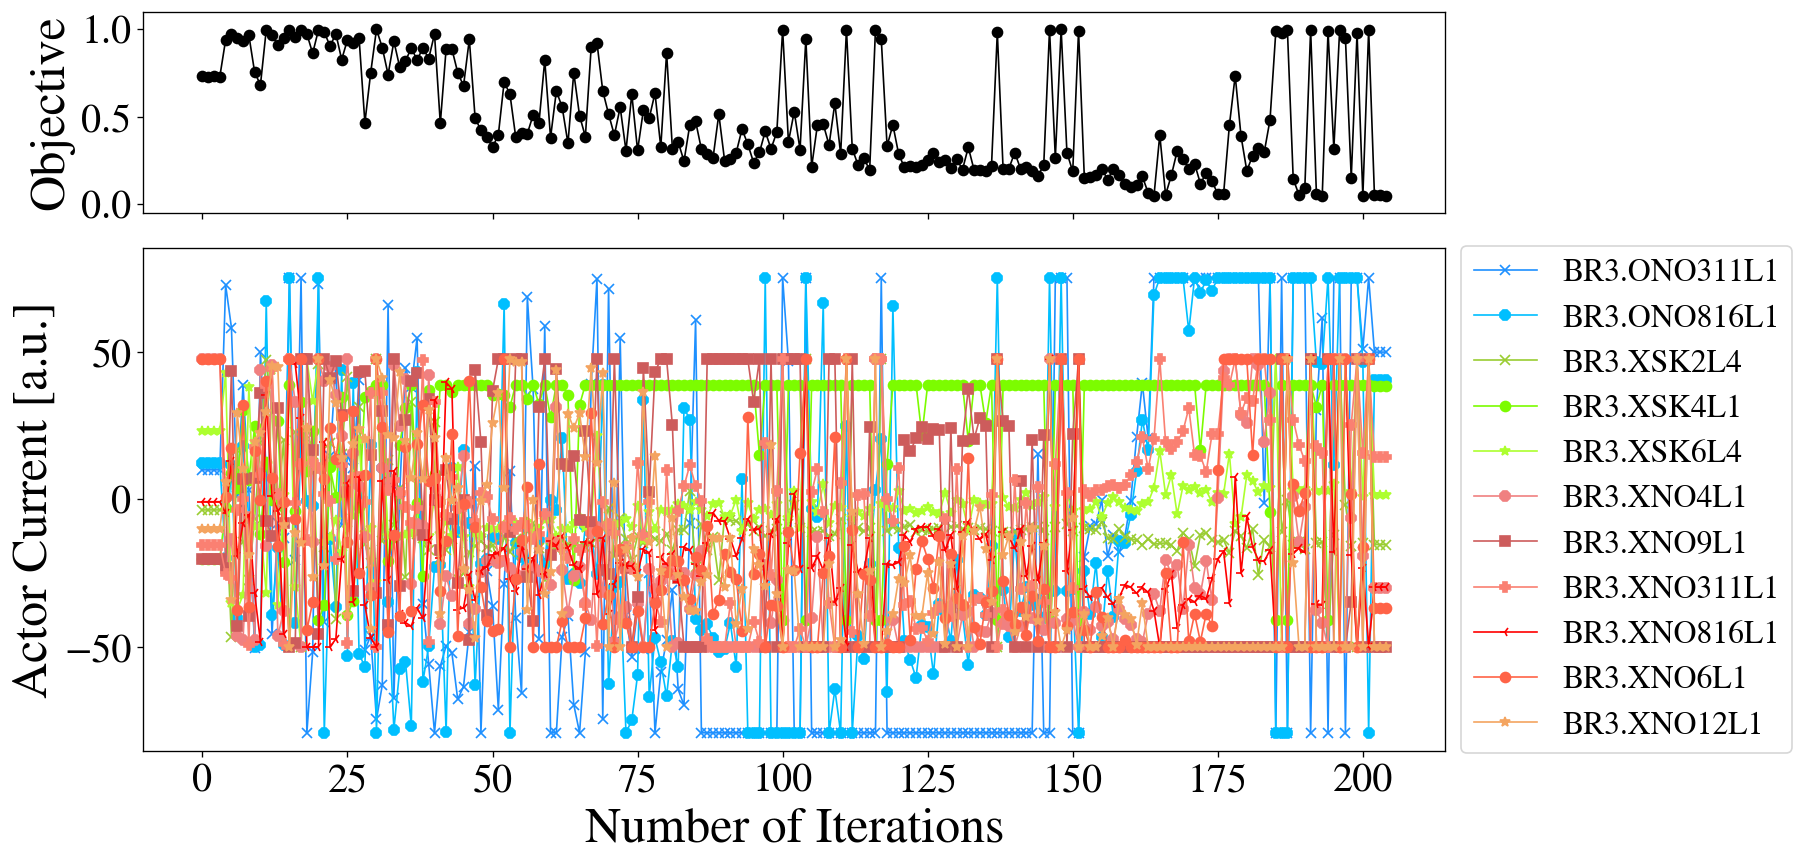
\includegraphics[width=\linewidth]{chapter5/2023_05_02_R3_LHCramp_BayesOpt.png}
    \caption{Summary for Bayesian optimization of resonance compensation applied to Ring 3 in the CERN PSB.}
    \label{fig:bo2}
\end{figure}

\subsection{BOBYQA (Bound Optimization BY Quadratic Approximation)}

\begin{figure}[H]
    \centering
    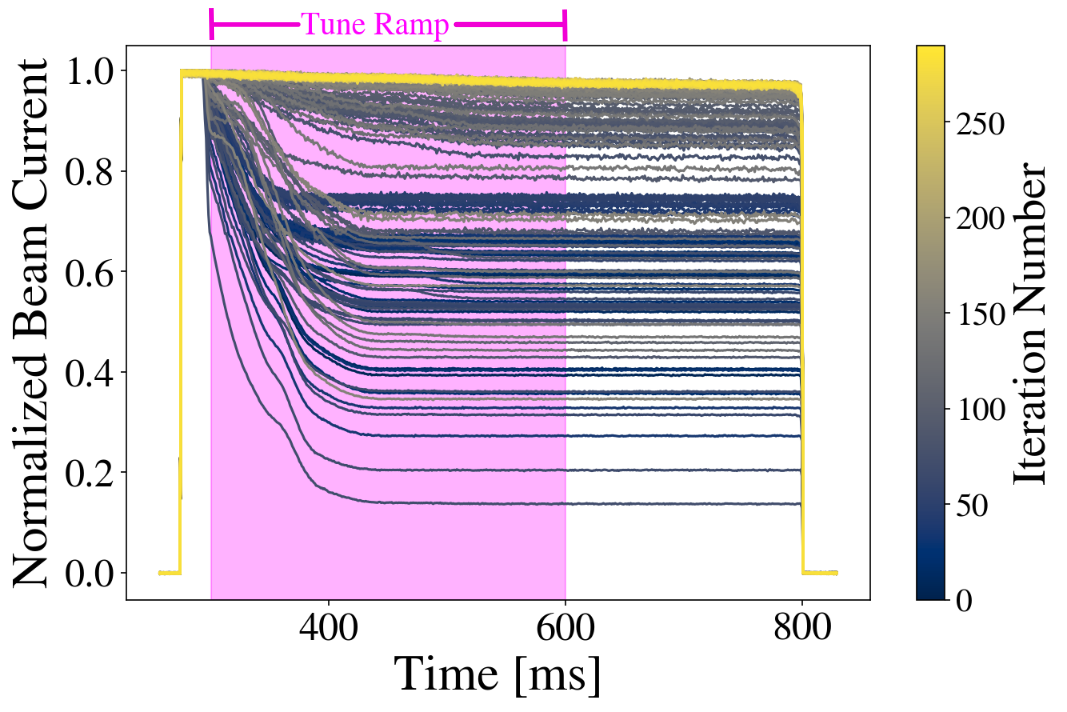
\includegraphics[width=\linewidth]{chapter5/i2_bobyqa_commented.png}
    \caption{Normalized beam current plots for the BOBYQA method done at Ring 1.}
    \label{fig:ibobyqa}
\end{figure}

\begin{figure}[H]
    \centering
    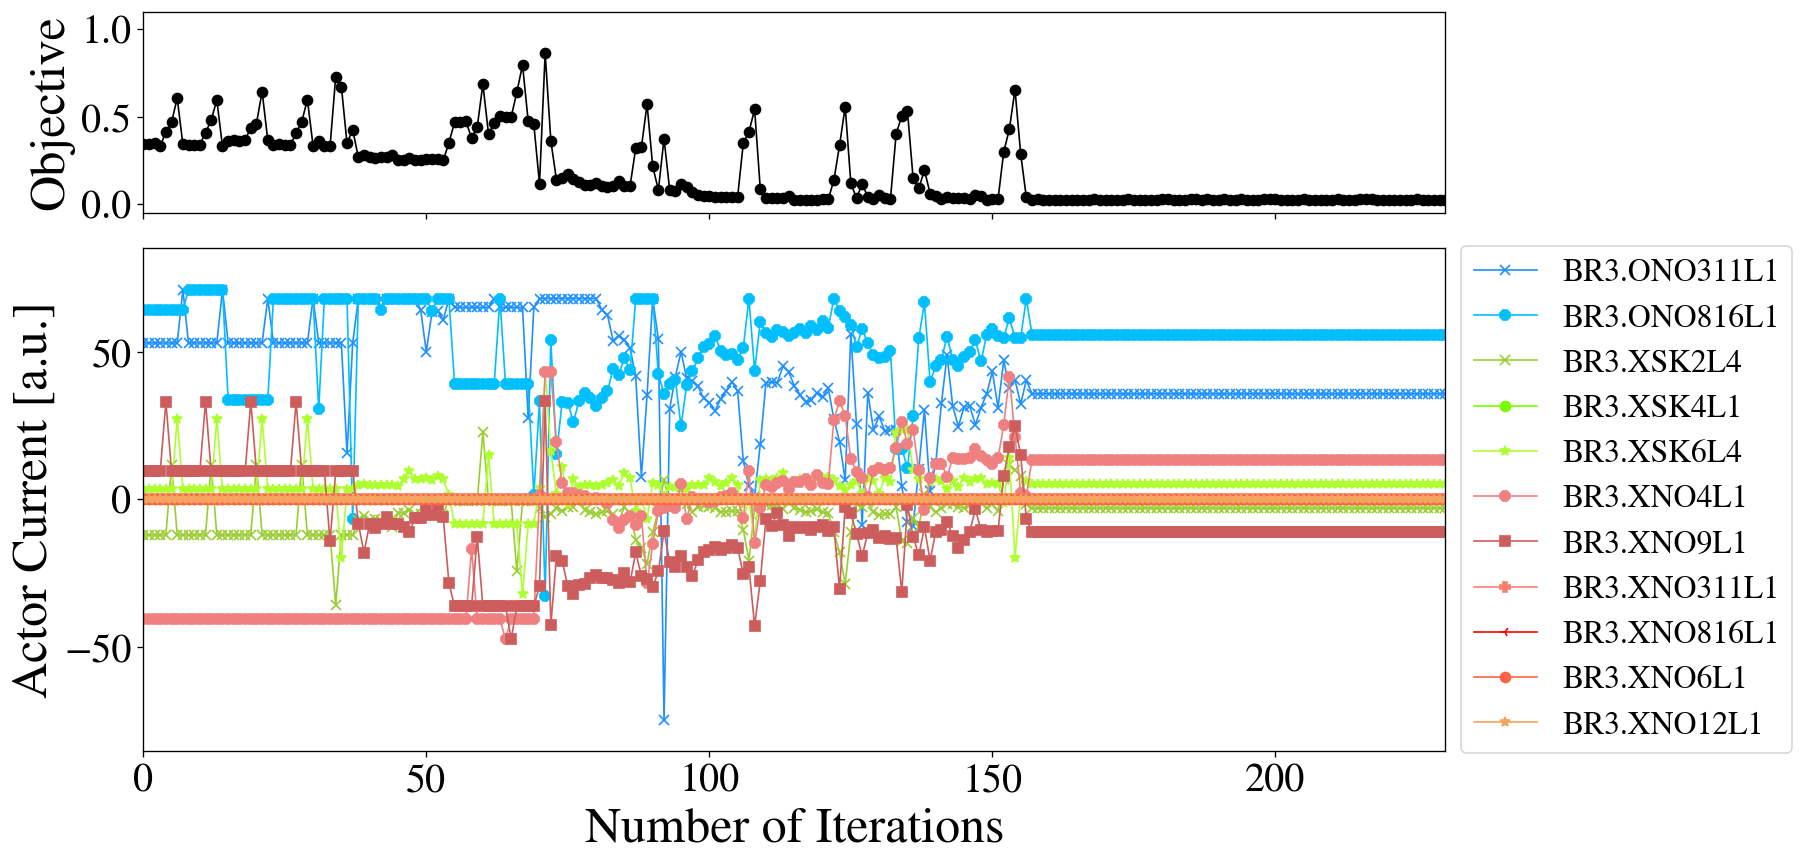
\includegraphics[width=\linewidth]{chapter5/2023_05_04_R3_BCMS_bobyqa.png}
    \caption{Summary for BOBYQA optimization of resonance compensation applied to Ring 3 in the CERN PSB for BCMS (Bunch Compression Merging and Splitting) beam.}
    \label{fig:bobyqa1}
\end{figure}

\section{Experimental Verification of Compensation}

\begin{figure}[H]
    \centering
    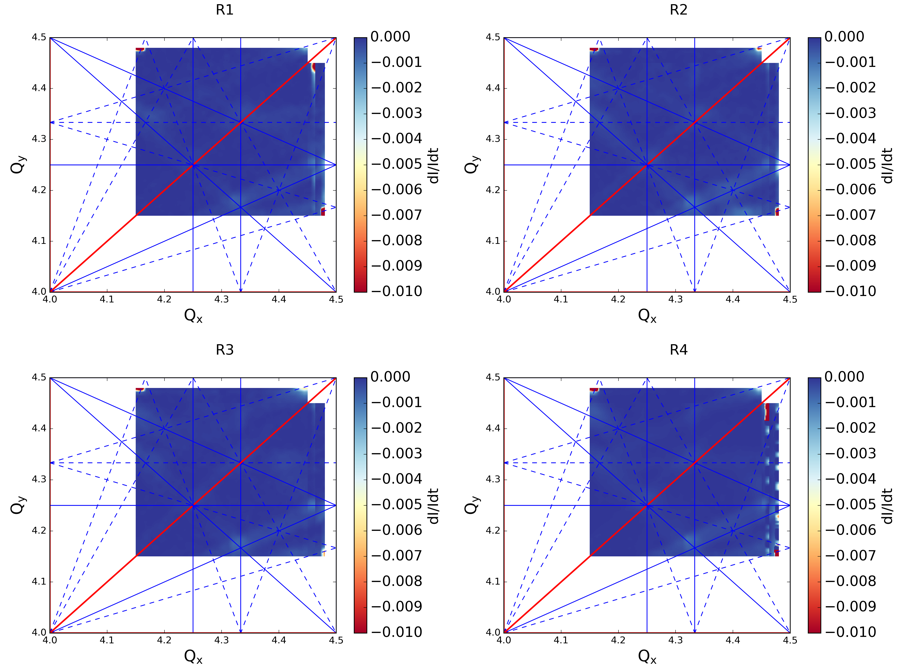
\includegraphics[width=\columnwidth]{chapter5/bocomp.png}
    \caption{Dynamic loss maps for the 4 rings in the PS Booster with the best configuration from the Bayesian optimization of the resonance compensation. The plots are an average of scanning in 4 directions.}
    \label{fig:bocomp_psb}
\end{figure}
